%---Linda

The accurancy of the post processed postions is decreasing with a increasing distance to the base station.
The nearest base station is Statens Kartverks SatRef located on Platåberget with a distance between 14 km and 20 km depending on the stake.\medskip

% 2 different methods:
In our report we use a new method for the postprocessing. 
This method is an open source alternative which is available for different system softwares. 
The previous used 'Trimble Business Center' software is only available on a windows system and needs a licens. 
We operate both methods to show that the results of both methods do not differ.
This approves that our results are comparable to the reuslts of the last years.\medskip

% steps of the post processing:
While the post processing with the usual method in the 'Trimble Business Center' all steps from section 5 in Gölles (2012) are done.
For each day the data file from the measurements and the corresponding base station data file is imported. 
We have data for the days of year (doy) 070, 072, 074 and 075.
All files from the base station are in the .o18-format. 
The data from the reciever have the .t02 format. 
After the post processing the results from the are stored in a .csv-file.\medskip

The open source post processing requires different steps.
First of all the raw data file has to be transformed from the .t02-format to the .tdg-format. 
The Trimble format .t02 is not readable for the final post processing program.
This was done with the programm rubpkr00 which is available on the website of unavco (http://kb.unavco.org/kb/article/trimble-runpkr00-v5-40-latest-version-mac-osx-10-7-windows-xp-7-linux-solaris-744.html).
The used command is 'runpkr00 -g -d filename.t02'.
Due to problems with the package we had to do a manual transformation of the package.
To provide the correct file format for the last post processing step we use the toolkit teqc.
This toolkit is also available on the website of unavco (https://www.unavco.org/software/data-processing/teqc/teqc.html).
Then the file can be converted by another commad using './teqc +nav filename.nav +obs filename.obs filename.tgd' to an observation (.obs) and navigation (.nav) file.
After that it is necessary to download also the base station data from the platform http://ftp.statkart.no/.
The final step in the post processing of the GPS data is done with the open source program package RTKLIB.
This package is available for the download in the website http://www.rtklib.com/rtklib.htm.
In this package we use the executable rtkpost.exe in the subdirectory /bin of the downloaded full package with source Programs with the version 2.4.2.
In this software the two navigation file from the receiver and the base station as well as the observation file from the receiver has to be read in.
For this method the .n18-format from the basestation is needed as comparable navigation file.
The next steps are consistent to the description on the website https://docs.emlid.com/reach/common/tutorials/gps-post-processing/.
For this we had to modify the settings of rtkpost.exe and load the three required files. 
The final output after the post processing is a position file (.pos). 
This file includes for every time step the post processed position in longitude and latitude.
Then we calculate a median over all time steps to get an average position for every measurement.
Because we consistenly use the UTM coordinate system, we transform the lon/lat coordinates by using the python function from\_latlon.
The analysis in this report is made with python.\medskip

% error correction of the post processed data:
The post processed data are not the final data. 
To get the final position with a minimal error to the real position, we have to include the different aspects from our measurement setup (see section setup).
We subtract the distance between the rover and the stake from the northing component.
In addition, we consider the inclination of the stake and calculate the error dependent on the height of the stake and the direction of the inclination.\medskip

\begin{figure}
\centering
\includegraphics[width=\linewidth]{../pictures/schematic_setup.pdf}
\caption{Schematic figure of the relevant parameter in the measurment setup.}
\end{figure}


\begin{equation}
	\Delta_{abs} = (h_{snow} + h_{antenna} - h_{ref_year}) * sin(\alpha)
\end{equation}

\begin{equation}
	\Delta_{north} = - \Delta_{abs} * cos(\phi)
\end{equation}

\begin{equation}
	\Delta_{east} = - \Delta_{abs} * sin(\phi)
\end{equation}

% name accurancies of the final data:
Despite all the correction, it is important for the interpretation of the results to consider the accurancy of all parts our measurments.

% tables:
\begin{table}[h]
\caption{Final positions after the TBC post processing.}
\centering 
\begin{tabular}{lrrr}
\toprule
        Name &  Northing [m] &  Easting [m] &  Elevation [m] \\
\midrule
    BL2-2016 &    8686150.51 &    523049.54 &         436.86 \\
    BL2-2018 &    8686149.27 &    523051.55 &         437.76 \\
    BL3-2016 &    8686092.71 &    523543.82 &         491.07 \\
    BL3-2018 &    8686091.13 &    523545.37 &         491.15 \\
    BL4-2018 &    8686098.89 &    524181.02 &         571.86 \\
  BL4-i-2016 &    8686099.66 &    524179.06 &         571.55 \\
 BL4-ii-2016 &    8686099.30 &    524179.33 &         571.36 \\
  BL5-i-2017 &    8686129.64 &    524644.30 &         628.64 \\
 BL5-ii-2017 &    8686129.44 &    524644.29 &         628.61 \\
     T1-2018 &    8687106.61 &    528388.32 &         341.43 \\
   T1-i-2017 &    8687105.34 &    528388.87 &         341.25 \\
  T1-ii-2017 &    8687105.06 &    528388.51 &         341.30 \\
     T2-2016 &    8687320.86 &    527951.55 &         395.12 \\
     T2-2018 &    8687319.67 &    527950.59 &         395.13 \\
   T2-i-2017 &    8687320.99 &    527951.91 &         395.17 \\
  T2-ii-2017 &    8687320.68 &    527951.29 &         395.25 \\
     T3-2017 &    8687273.10 &    527598.30 &         422.57 \\
     T4-2016 &    8687141.52 &    527123.96 &         486.78 \\
     T4-2018 &    8687137.40 &    527124.77 &         487.25 \\
     T5-2016 &    8686935.92 &    526692.26 &         534.57 \\
     T5-2018 &    8686937.70 &    526690.76 &         535.26 \\
     T6-2016 &    8686673.29 &    526248.19 &         561.86 \\
     T6-2018 &    8686674.33 &    526246.57 &         560.49 \\
     T7-2015 &    8686581.42 &    525859.20 &         615.80 \\
     T7-2017 &    8686579.33 &    525858.40 &         615.81 \\
     T8-2017 &    8686470.03 &    525522.18 &         649.70 \\
\bottomrule
\end{tabular}

\end{table}

%\begin{table}[h]
%\caption{Final positions after the open source post processing.}
%\centering
%\begin{tabular}{lcccccc}
\toprule
        Name &           Northing [m] &           Easting [m] &      Elevation [m] \\
\midrule
    BL2-2016 &  8686150.74 $\pm$ 0.16 &  523049.41 $\pm$ 0.11 &  436.89 $\pm$ 0.48 \\
    BL2-2018 &  8686149.82 $\pm$ 0.02 &  523051.47 $\pm$ 0.03 &  437.74 $\pm$ 0.06 \\
    BL3-2016 &  8686091.51 $\pm$ 0.27 &  523544.75 $\pm$ 0.13 &  490.82 $\pm$ 0.25 \\
    BL3-2018 &  8686091.17 $\pm$ 0.42 &  523545.34 $\pm$ 0.10 &  491.39 $\pm$ 1.03 \\
    BL4-2018 &  8686098.89 $\pm$ 0.21 &  524181.02 $\pm$ 0.20 &  570.94 $\pm$ 0.20 \\
  BL4-i-2016 &  8686098.47 $\pm$ 0.27 &  524179.80 $\pm$ 0.19 &  571.65 $\pm$ 0.20 \\
 BL4-ii-2016 &  8686098.39 $\pm$ 1.30 &  524179.92 $\pm$ 0.31 &  571.36 $\pm$ 4.82 \\
  BL5-i-2017 &  8686130.74 $\pm$ 0.09 &  524644.27 $\pm$ 0.01 &  628.63 $\pm$ 0.09 \\
 BL5-ii-2017 &  8686130.74 $\pm$ 0.28 &  524644.28 $\pm$ 0.15 &  628.56 $\pm$ 0.75 \\
     T1-2018 &  8687106.55 $\pm$ 0.32 &  528388.42 $\pm$ 0.07 &  341.59 $\pm$ 0.24 \\
   T1-i-2017 &  8687105.69 $\pm$ 0.13 &  528388.68 $\pm$ 0.18 &  341.26 $\pm$ 0.12 \\
  T1-ii-2017 &  8687105.58 $\pm$ 0.45 &  528388.84 $\pm$ 0.44 &  341.38 $\pm$ 0.65 \\
     T2-2016 &  8687321.31 $\pm$ 0.42 &  527951.88 $\pm$ 0.14 &  394.88 $\pm$ 2.34 \\
     T2-2018 &  8687319.62 $\pm$ 0.28 &  527951.35 $\pm$ 0.27 &  395.86 $\pm$ 1.61 \\
   T2-i-2017 &  8687321.37 $\pm$ 0.30 &  527950.58 $\pm$ 0.25 &  395.22 $\pm$ 0.34 \\
  T2-ii-2017 &  8687320.98 $\pm$ 1.31 &  527951.01 $\pm$ 0.26 &  394.74 $\pm$ 1.26 \\
     T3-2017 &  8687273.11 $\pm$ 0.12 &  527598.29 $\pm$ 0.01 &  422.59 $\pm$ 0.07 \\
     T4-2016 &  8687138.56 $\pm$ 0.47 &  527123.97 $\pm$ 0.34 &  486.80 $\pm$ 1.07 \\
     T4-2018 &  8687137.72 $\pm$ 1.05 &  527124.90 $\pm$ 0.37 &  487.94 $\pm$ 2.33 \\
     T5-2016 &  8686938.28 $\pm$ 0.57 &  526692.25 $\pm$ 0.25 &  534.57 $\pm$ 0.72 \\
     T5-2018 &  8686937.68 $\pm$ 0.21 &  526690.76 $\pm$ 0.21 &  535.09 $\pm$ 0.45 \\
     T6-2016 &  8686675.01 $\pm$ 0.51 &  526250.17 $\pm$ 0.22 &  561.87 $\pm$ 0.89 \\
     T6-2018 &  8686674.78 $\pm$ 0.48 &  526246.88 $\pm$ 0.39 &  560.47 $\pm$ 0.79 \\
     T7-2015 &  8686580.26 $\pm$ 0.26 &  525857.56 $\pm$ 0.26 &  613.96 $\pm$ 0.71 \\
     T7-2017 &  8686579.37 $\pm$ 0.19 &  525858.38 $\pm$ 0.04 &  615.95 $\pm$ 0.71 \\
     T8-2017 &  8686471.52 $\pm$ 0.48 &  525523.82 $\pm$ 0.13 &  649.73 $\pm$ 1.02 \\
\bottomrule
\end{tabular}

%\end{table}

The raw data from our measurements are given in the appendix (table xy). 
%\usepackage{pdflscape}
%\begin{landscape}
%\begin{table}[h]
%\caption{Raw data collected in the field.}
%\centering
%\begin{tabular}{lllllllll}
\toprule
        Name & Northing [m] & Easting [m] & Elevation [m] & Antenna height [m] & Snow depth [m] & Inclination [deg] & Direction of Incl. [deg] & Distance Rover-Stake [m] \\
\midrule
    BL2-2016 &   8686150.91 &   523049.58 &        441.45 &               2.18 &            1.1 &                 3 &                      225 &                     0.18 \\
    BL2-2018 &   8686149.18 &   523052.26 &         439.6 &                0.6 &              0 &                 2 &                      270 &                        0 \\
    BL3-2016 &   8686090.70 &   523545.65 &        486.42 &                2.2 &           1.07 &                12 &                      270 &                      0.1 \\
    BL3-2018 &   8686090.05 &   523546.95 &        485.58 &                0.6 &              0 &                 0 &                        0 &                        0 \\
    BL4-2018 &   8686100.72 &   524179.05 &        569.47 &               0.92 &              0 &                 0 &                        0 &                        0 \\
  BL4-i-2016 &   8686098.16 &   524180.50 &        577.73 &               2.08 &           0.93 &                10 &                      270 &                     0.11 \\
 BL4-ii-2016 &   8686099.46 &   524180.49 &        575.12 &               1.25 &           1.25 &                10 &                      270 &                      0.2 \\
  BL5-i-2017 &   8686132.09 &   524644.27 &         631.4 &               1.32 &            1.1 &                 0 &                        0 &                      1.1 \\
 BL5-ii-2017 &   8686128.59 &   524645.35 &        624.69 &               0.48 &            1.3 &                 0 &                        0 &                      1.3 \\
     T1-2018 &   8687106.45 &   528388.09 &        343.82 &               0.66 &              0 &                 0 &                        0 &                        0 \\
   T1-i-2017 &   8687106.51 &   528389.87 &         342.4 &                2.2 &            0.8 &                 9 &                      180 &                     0.15 \\
  T1-ii-2017 &   8687104.86 &   528388.57 &         340.5 &               2.15 &            0.8 &                10 &                      180 &                     0.17 \\
     T2-2016 &   8687322.63 &   527951.49 &        400.25 &               1.34 &           0.97 &                 0 &                        0 &                      0.1 \\
     T2-2018 &   8687318.62 &   527951.78 &        391.96 &               0.66 &              0 &                 5 &                      225 &                        0 \\
   T2-i-2017 &   8687321.16 &   527951.98 &        393.06 &               2.23 &              1 &                10 &                       90 &                      0.1 \\
  T2-ii-2017 &   8687321.10 &   527952.02 &         396.3 &                1.4 &              1 &                 5 &                      135 &                      0.1 \\
     T3-2017 &   8687273.68 &   527599.16 &        428.93 &               1.87 &           1.05 &                 0 &                        0 &                      0.1 \\
     T4-2016 &   8687138.55 &   527125.09 &         490.1 &               2.42 &            1.2 &                 5 &                        0 &                      0.1 \\
     T4-2018 &   8687138.56 &   527125.09 &         490.1 &               0.63 &              0 &                 0 &                        0 &                        0 \\
     T5-2016 &   8686940.26 &   526691.93 &        538.15 &               2.44 &           1.22 &                 8 &                        0 &                      0.1 \\
     T5-2018 &   8686939.86 &   526689.56 &        548.25 &               0.45 &              0 &                 0 &                        0 &                        0 \\
     T6-2016 &   8686676.52 &   526249.39 &        568.05 &                2.3 &           1.35 &                 4 &                      180 &                     0.15 \\
     T6-2018 &   8686673.79 &   526246.38 &        559.77 &               1.95 &            1.4 &                 0 &                        0 &                        0 \\
     T7-2015 &   8686579.41 &   525858.64 &        612.84 &               1.84 &            1.2 &                10 &                       45 &                      0.1 \\
     T7-2017 &   8686378.63 &   525858.64 &        615.19 &               0.98 &           1.21 &                 0 &                        0 &                        0 \\
     T8-2017 &   8686471.63 &   525524.23 &        650.45 &               2.09 &            0.7 &                 5 &                      180 &                      0.1 \\
\bottomrule
\end{tabular}

%\end{table}
%\end{landscape}


